% -*- mode: fundamental -*-

% ****************************************************************

\chapter{RISC-V: the Fife pipelined CPU}

\markboth{Ch \arabic{chapter}: Pending (DRAFT)}{\copyrightnotice}

\setcounter{page}{1}
% \renewcommand{\thepage}{\arabic{page}}
\renewcommand{\thepage}{\arabic{chapter}-\arabic{page}}

\label{ch_Fife_Pending}

% ****************************************************************

\section{Introduction}

In this chapter we turn our attention to Fife, the pipelined CPU.  We
will reuse all the code already developed for Drum that implements
basic RISC-V semantics.  Our focus here is purely on pipelining and
solving the new problems raised by pipelining.

Figure~\ref{Fig_Instr_Exec_w_FIFOs} annotates the abstract execution
algorithm in Figure~\ref{Fig_Instr_Exec} with some specifics for the
pipelined implementation in Fife.
\begin{figure}[htbp]
  \centerline{\includegraphics[width=6in,angle=0]{Figures/Fig_Instr_Exec_w_FIFOs}}
  \caption{\label{Fig_Instr_Exec_w_FIFOs}Pipelined interpretation of RISC-V instructions (Fig.~\ref{Fig_Instr_Exec} with new annotations)}
\end{figure}
Unlike Drum, where each yellow box was one step in a sequential
process, now we interpret each yellow box as containing its own
infinite process.  There are now half-a-dozen or more processes in the
diagram (one for each yellow box), all running \emph{concurrently}.

For each of the yellow boxes, we use the word ``\emph{step}'' for Drum
and ``\emph{stage}'' for Fife.  For Fife, each black arrow in the
diagram represents a flow of \emph{messages} sent from one stage to
another.  These messages are sent via FIFO buffers (depicted by
\raisebox{-0.2ex}{
\includegraphics[width=0.2in,angle=0]{Figures/Fig_FIFO}}
annotations in the figure).

Each stage is an infinite loop, consuming incoming messages and
producing outgoing messages.  Thus, while the Retire stage is working
on instruction $n$, the Execute, Register-Read, Decode and Fetch
stage(s) may be working on instructions $n+1$, $n+2$, $n+3$, and
$n+4$, respectively.  Thus, there is a sequence, or train, of
instructions flowing through the diagram from left to right.

Pipelining raises four new problems, and these are the focus of this
chapter:

\begin{itemize}

  \item Keeping the Fetch Stage Working with PC Prediction and Epochs

  \item Managing Register Read/Write Hazard with a Scoreboard

  \item Retiring outputs of the Execute Stages in Order with Tags

  \item Allowing Memory Ops to be Pipelined with a Store Buffer

\end{itemize}

% ****************************************************************

\section{Keeping the Fetch Stage Working with PC Prediction and Epochs}

What should the Fetch stage do after issuing a request to IMem for
instruction $n$?  To issue another request, it needs to know the PC of
instruction $n+1$, but there are several uncertainties about that next
PC:

\begin{tightlist}

 \item The current Fetch itself can raise an exception (trap) if its
        PC is misaligned, is an unsupported memory address, {\etc}.
        In this case the next PC will the trap-handler PC instead of
        the ``normal'' next PC.

 \item If it is a BRANCH instruction, until it reaches the Execute
       Control stage we do not know the branch target PC address, nor
       if the branch is taken or not.

 \item If it is a JAL or JALR instruction, until it reaches the
       Execute Control stage we do not know the target PC address.

 \item Many instructions can raise an exception (trap) (illegal
       instructions, BRANCH/JAL/JALR with misaligned target addresses,
       DMem ops with misaligned addresses or unsupported addresses,
       {\etc}); in these cases the next PC will the trap-handler PC
       instead of the ``normal'' next PC.

 \item The CPU may choose to respond to an external interrupt, in
        which case the next PC will be the interrupt-handler's
        address.

\end{tightlist}

Note, the Fetch stage knows nothing about instruction $n$ other than
its PC.  The instruction itself is not known until IMem sends its
response to the Decode stage (and assuming the Fetch does not raise an
exception).

% ================================================================

\subsection{PC Prediction in the Fetch Stage}

\index{RISCV!Branch prediction}
\index{RISCV!PC prediction}
\index{RISCV!Prediction}
\index{RISCV!Misprediction (wrong path instructions)}
\index{RISCV!Wrong-path due (mispredicted instructions)}

A standard solution is for the Fetch stage to \emph{predict} the next
PC, {\ie} make a guess about the next PC.  Since all RISC-V RV32
instructions are 32-bits wide (4 bytes), and \emph{most} of them
``fall-through'' to the next adjacent instruction, a simple prediction
is: PC+4.  This prediction will be correct for most instructions, but
will be wrong for BRANCH instructions that take the branch, for
JAL/JALR instructions, and for any instruction that traps.  When the
prediction is wrong, the instructions that follow immediately are
called ``mispredicted'' or ``wrong-path'' instructions.

% ----------------
\vspace{2ex}

NOTE:
\fbox{\small
\begin{minipage}{5in}

RISC-V instructions are all 32-bits wide, so PC+4 is a reasonably good
guess.  In ISAs that have variable-length instructions, prediction may
be more complicated.  Even in RISC-V, when implementing the ``C''
(Compressed Instructions) extension, some instructions may be 16-bits
wide, raising similar complications.

\vspace{1ex}

Earlier we said ``the Fetch stage knows nothing about instruction $n$
other than its PC''.  This is not strictly true--the CPU may have
fetched this PC before ({\eg} this PC is inside a loop, or in a
procedure that is called repeatedly).  Knowledge of past behavior can
improve the current prediction.  Most predictors in modern processors
use past history to improve and ``tune'' their branch predictors
dynamically while executing the program.  Designing good branch
predictors is a deep topic for which there are many good textbooks
(for example, \cite{Hennessy2017}).

\vspace{1ex}

PC prediction can be seen as a kind of ``machine learning''.  The
CPU's past execution history constitutes the ``training data'' for a
model, and the model is then asked to predict the next PC for the
current PC.

\end{minipage}}
% ----------------

% ================================================================

\subsection{Identifying and Flushing Wrong-path Instructions}

Clearly, we need to identify and flush wrong-path instructions from
the pipeline.

Suppose the Fetch stage issues requests for two instructions $i_1$ at
address $a_1$ and $i_2$ at address $a_2$, where $a_2$ is predicted
from $a_1$.  When issuing the request for $a_1$, the Fetch stage can
pass along $a_2$ to the Decode stage, from which point it can
accompany $i_1$ as it journeys through the pipeline ({\ie} every
instruction is accompanied by its next-PC prediction).

When $i_1$ reaches the Retire stage, we know the \emph{correct} next
PC (Trap handler PC?  PC+4?  Branch-taken target?  JAL/JALR target?).
By comparing this actual next PC with $a_2$, we know whether the
successor to $i_1$ was predicted correctly or not.

If we find that the prediction was correct, there is nothing more to
be done; we allow the pipeline flow to proceed.

\index{RISCV!PC prediction!redirection}
\index{RISCV!redirection on misprediction}

If we find that the prediction was wrong, then two things must happen:

\begin{itemize}

  \item We need to \emph{redirect} the Fetch stage to start fetching
    from the correct next-PC.  This involves sending a message from
    the Retire stage back to the Fetch stage containing the correct
    next-PC.  Suppose the first instruction fetched after this
    redirection is $j_1$.

  \item Instruction $i_2$, and possibly following instructions $i_3$,
    $i_4$, ... until $j_1$ are wrong-path instructions, and must be
    flushed.

\end{itemize}

\index{RISCV!rg\_epoch@{\tt rg\_epoch} register for managing mispredictions}

When the Retire stage starts flushing wrong-path instructions $i_2$,
$i_3$, $i_4$, ... how does it know when it has reached the end of the
wrong-path sequence?  In other words, how does it know when it sees
$j_1$?  This is precisely the purpose of the \verb|rg_epoch| register
shown in Figure~\ref{Fig_Instr_Exec_w_FIFOs}.

Think of \verb|rg_epoch| as a counter that continuously counts upward.
Suppose the current value is $e_1$.  As described above, when the
Retire stage recognizes an instruction whose successor has been
mispredicted, we send a redirection message to the Fetch stage with
the corrected PC. The Retire stage also increments $e_1$ and sends the
incremented value as part of the redirection.  Each time the Fetch
stage is redirected, it remembers the new epoch value.  It also sends
this value down the pipeline, accompanying each instruction fetched
with this value.

Now, flushing wrong-path instructions in the Regire stage is easy:
$i_2$, $i_3$, $i_4$, ... will be accompanied by the old epoch value
$e_1$, whereas the first correct-path instruction $j_1$ will be
accompanied by the new epoch value $e_1+1$.  Thus, the Retire stage
knows exactly which instructions are wrong-path and it can discard
them.

% ----------------
\hdivider

\Exercise

We have describe \verb|rg_epoch| as a counter that is incremented on
each recognition of a misprediction.  If the register contents have
type \verb|Bit #(n)|, then this will wrap-around to 0 after $2^n$
increments.  Is this a problem?

\Exercise

If \verb|rg_epoch| contains a \verb|Bit #(n)| value, how small can $n$ be?

\Endexercise
% ----------------

% ================================================================

\subsection{Mispredicted instructions should not have any side-effects}

It is not enough for the Retire stage just to discard mispredicted
instructions.  Instructions have side-effects: they may modify
registers and write to memory.  We must ensure that mispredicted
instructions make no modifications that are visible to right-path
instructions that follow.  The details of how this is accomplished
will be seen in Section~\ref{Sec_Store_Buffers} and
Section~\ref{Sec_Retire_Stage}.

% ****************************************************************

\section{Managing Register Read/Write Hazards with a Scoreboard}

\label{Sec_Scoreboards}

Suppose instruction $i_1$ writes to register $x_7$, and the following
instruction $i_2$ reads from register $x_7$.  Instruction $i_1$'s
write to $x_7$ only happens in the Retire stage.  If $i_2$ were to
follow behind $i_1$ immediately, it will be in the Exec stage, and
would have already read $x_7$ earlier when it was in the Register-Read
stage.  In other words, it would have read a \emph{stale} or obsolete
value $x_7$.  This is called a Read-Write \emph{hazard}, or a
read-after-write \emph{dependency}.

In this situation, we need to make $i_2$ wait in the Register-Read
stage until $i_1$ has completed its update of $x_7$.  This is
precisely the purpose of the \verb|scoreboard| shown in
Figure~\ref{Fig_Instr_Exec_w_FIFOs}.

The \verb|scoreboard| is an array of 32 1-bit registers (one bit for
each GPR).  When an instruction (such as $i_1$) passes through the
Register-Read stage, if it writes to register $x_7$, we set the
corresponding bit 7 in the scoreboard to 1, indicating that $x_7$ is
``busy''.  When $i_1$ reaches the Retire stage and writes to the
register, it also resets the scoreboard bit 7 to 0, indicating that
$x_7$ is ``not busy''.

When an instruction (such as $i_2$) reaches the Register-Read stage
and wants to read a register (such as $x_7$), if the corresponding
scoreboard bit says it is busy, then the Register-Read stage
``\emph{stalls}'', {\ie} it waits until the scoreboard condition is
cleared (by $i_1$ in the Retire stage).

\index{RISCV!Pipeline!Bubble}
\index{RISCV!Bubble in a pipeline}

While $i_2$ is waiting in the stalled Register-Read stage, note that
the following Execute stage may become ``empty'', {\ie} there is no
instruction occupying that stage.  We refer to this as a
``\emph{pipeline bubble}''.

% ----------------
\hdivider

\Exercise

For two consecutive instructions $i_1$ and $i_2$,
  \begin{tightlist}
    \item $i_1$ may want to write register $x_7$ and $i_2$ may want to read $x_7$,
    \item $i_1$ may want to write register $x_7$ and $i_2$ may write to write $x_7$,
    \item $i_1$ may want to read register $x_7$ and $i_2$ may want to read $x_7$,
    \item $i_1$ may want to read register $x_7$ and $i_2$ may want to write $x_7$.
  \end{tightlist}
Above, we motivated scoreboards with the first scenario.  What about
the other three scenarios?

\Exercise

Write-write hazards can be treated just like read-after-write hazards.
Alternatively the 1-bit in the scoreboard for a register (say $x_7$)
can be generalized into an $n$ bit up/downcounter, indicating the
number of instructions that have been allowed into Execute pipelines
that intend to write $x_7$.  The Retire stage decrements this counter;
the Register-Read stage stalls an instruction if these counters (for
its input registers) are non-zero; and the Register-Read stage
increments this counter for an instruction's destination register.

\vspace{1ex}

Implement a scoreboard module with this scheme.  What should happen if
a counter reaches its maximum value?  How many bits should each
counter have?

\vspace{1ex}

\Exercise

In the counter-based scoreboard of the previous exercise, if there are
multiple instructions in the Execute stages that intend to write
$x_7$, in what order can those writes occur?  What would be the
consequences of a wrong order?

\emph{Hint:} The answer is in Section~\ref{Sec_Reorder_Tags}.

\Endexercise
% ----------------

% ----------------------------------------------------------------

\subsubsection{Bypassing}

\index{RISCV!Bypassing}
\index{RISCV!Short-circuiting (bypassing)}

Digital hardware usually runs in time units of ``clock cycles''.  The
Retire stage writes a GPR (possibly) and writes the scoreboard (to
mark it ``not-busy'').  The Register-Read stage reads zero to two
GPRs, reads the scoreboard (to check ``not-busy'') and writes the
scoreboard (to set ``busy'').

\vspace{1ex}

For ordinary registers a write is only visible on the next clock
cycle.  Thus, if the scoreboard is just an ordinary register, the
Register-Read stage cannot observe ``not-busy'' until one clock after
the Retire stage has marked ``not-busy''.  This does not affect
correctness, but slows the performance of the CPU.

\vspace{1ex}

It is possible to design some extra circuitry around the scoreboard so
that the Register-Read stage can observe ``not-busy'' on the
\emph{same} clock cycle as when Retire marks it ``not-busy''.  This
technique is generically called ``\emph{bypassing}'' or
``\emph{short-circuiting}''.

% ----------------
\hdivider

\Exercise

Implement a scoreboard unit with bypassing/short-circuiting as
described in the above note.

\emph{Hint:} Needs BSV ``Concurrent Registers'' (advanced topic!)

\Exercise

What are the implications of bypassing/short-circuiting on the length
of combinational paths in a design, and the consequent effect on
achievable clock frequency?

\Endexercise
% ----------------

An even more advanced form of bypassing (with much more circuit
complexity) would be:

\begin{tightlist}

 \item Eliminate the scoreboard; do not stall an instruction in the
     Register-Read stage, but allow it to move into its appropriate
     Execute stage, and stall it there if necessary.  This frees up
     the Register-Read stage to process the next instruction, which
     may move into a different Execute stage.

 \item When Retire writes a register value, broadcast it to the
     different Execute stages to enable instructions there that are
     stalled on this register value.

\end{tightlist}

% ****************************************************************

\section{Retiring outputs of the Execute Stages in Order with Tags}

\label{Sec_Reorder_Tags}

In Figure~\ref{Fig_Instr_Exec_w_FIFOs}, each yellow box in the Execute
stage is an independent pipeline handling a certain subset of the
instruction set.  For example, ``Execute Control'' handles BRANCH, JAL
and JALR instructions. ``Execute Integer Arithmetic and Logic Ops''
handles LUI, AUIPC, and all arithmetic and logic instructions.  ``Exec
Mem Op'' handles LOAD and STORE instructions.  If we extend Fife to
handle the ``M'' ISA extension, we would have a pipeline for integer
multiply and divide instructions.  If we extend Fife to handle the
``F'' and ``D'' ISA extension, we would have a pipeline for floating
point arithmetic.  The Register-Read-and-Dispatch stage sends
information into these pipes depending on the kind of instruction.

Instructions may have different latencies in traversing these Execute
pipes.  For example, Control and Integer ops may typically traverse in
one clock, but multiplication, division, floating point and memory ops
may take more clocks.  The latency variation may be data dependent:
for example multiplication/division may recognize the special case
where an operand is 0 or 1 and return a result quickly.  A memory op
may return quickly on a cache hit, and take more time on a cache miss.

The Retire stage needs to gather the outpus from the Execute stages
and retire them in the proper order.  But, because of varying latency,
availability of data is not an indication of the proper order.

The solution to this ``ordering'' problem is \emph{tags}.  In
Figure~\ref{Fig_Instr_Exec_w_FIFOs} we see there is also a
\emph{direct path} from Register-Read-and-Dispatch to Retire.  We pass
a tag on this path \emph{for every instruction}.  For example if the
instruction is a BRANCH instruction, the Register-Read-and-Dispatch
stage sends information into Execute Control, but it also sends a tag
on the direct path to Retire indicating this, {\ie} that it has just
dispatched an instruction into Execute Control.

Thus, the sequence of tags on the direct path tells Retire exactly the
order in which to service the various Execute pipes.  For example, if
Retire sees a DMEM tag on the direct path, it knows that it must next
look for an output from the Exec Memory Ops pipe, even if outputs are
already available on the Execute Control and/or Execute Integer pipes.

% ****************************************************************

\section{Allowing Memory Ops to be Pipelined with a Store Buffer}

\label{Sec_Store_Buffers}

Instructions may attempt to write to memory. The {\tt store
    buffer} holds these updates until we can deterimine whether the
    instruction is a wrong-path instruction or not.  If it's a wrong
    path instruction, we can discard the update, else commit it to
    memory.

MMIO accesses may not be ``memory-like''.  A LOAD can have a
  side effect; a STORE may have side-effects more than just writing a
  value, such as starting a motor or launching a rocket!  Finally, a
  STORE to address $A$ followed by a LOAD from address $A$ may not
  return the same value.  For such accesses, the ``execute DMem''
  stage must defer the access until later when we are sure it is not a
  wrong-path instruction.

``Execute Memory Ops'' stage is always speculative (because of
mispredictions, and because older instructions in other pipes may
trap).

\begin{tightlist}
  \item Need for store-buffer and final commit/discard from Retire-stage
  \item Mem-system performs store only in store-buffer
  \item Retire stage sends commit/discard message to store-buffer.
        Discuss: do we need 'discard' messages, or are 'commit' messages enough?
\end{tightlist}

What about MMIO?

\begin{tightlist}
  \item LOADs may have side-effects
  \item LOADs may not be idempotent
  \item STOREs may have side-effects in addition to value stored
  \item LOAD may not return most-recently stored value
\end{tightlist}

So, these cannot be done speculatively, {\ie} in ``Execute Memory
Ops'' stage.

\begin{tightlist}

  \item 'Execute Memory ops' stage defers the request by sending it
    back as another kind of 'response'

  \item Retire step performs it once we know it is non-speculative.
\end{tightlist}


% ****************************************************************

\section{The Retire Stage}

\label{Sec_Retire_Stage}

\begin{figure}[htbp]
  \centerline{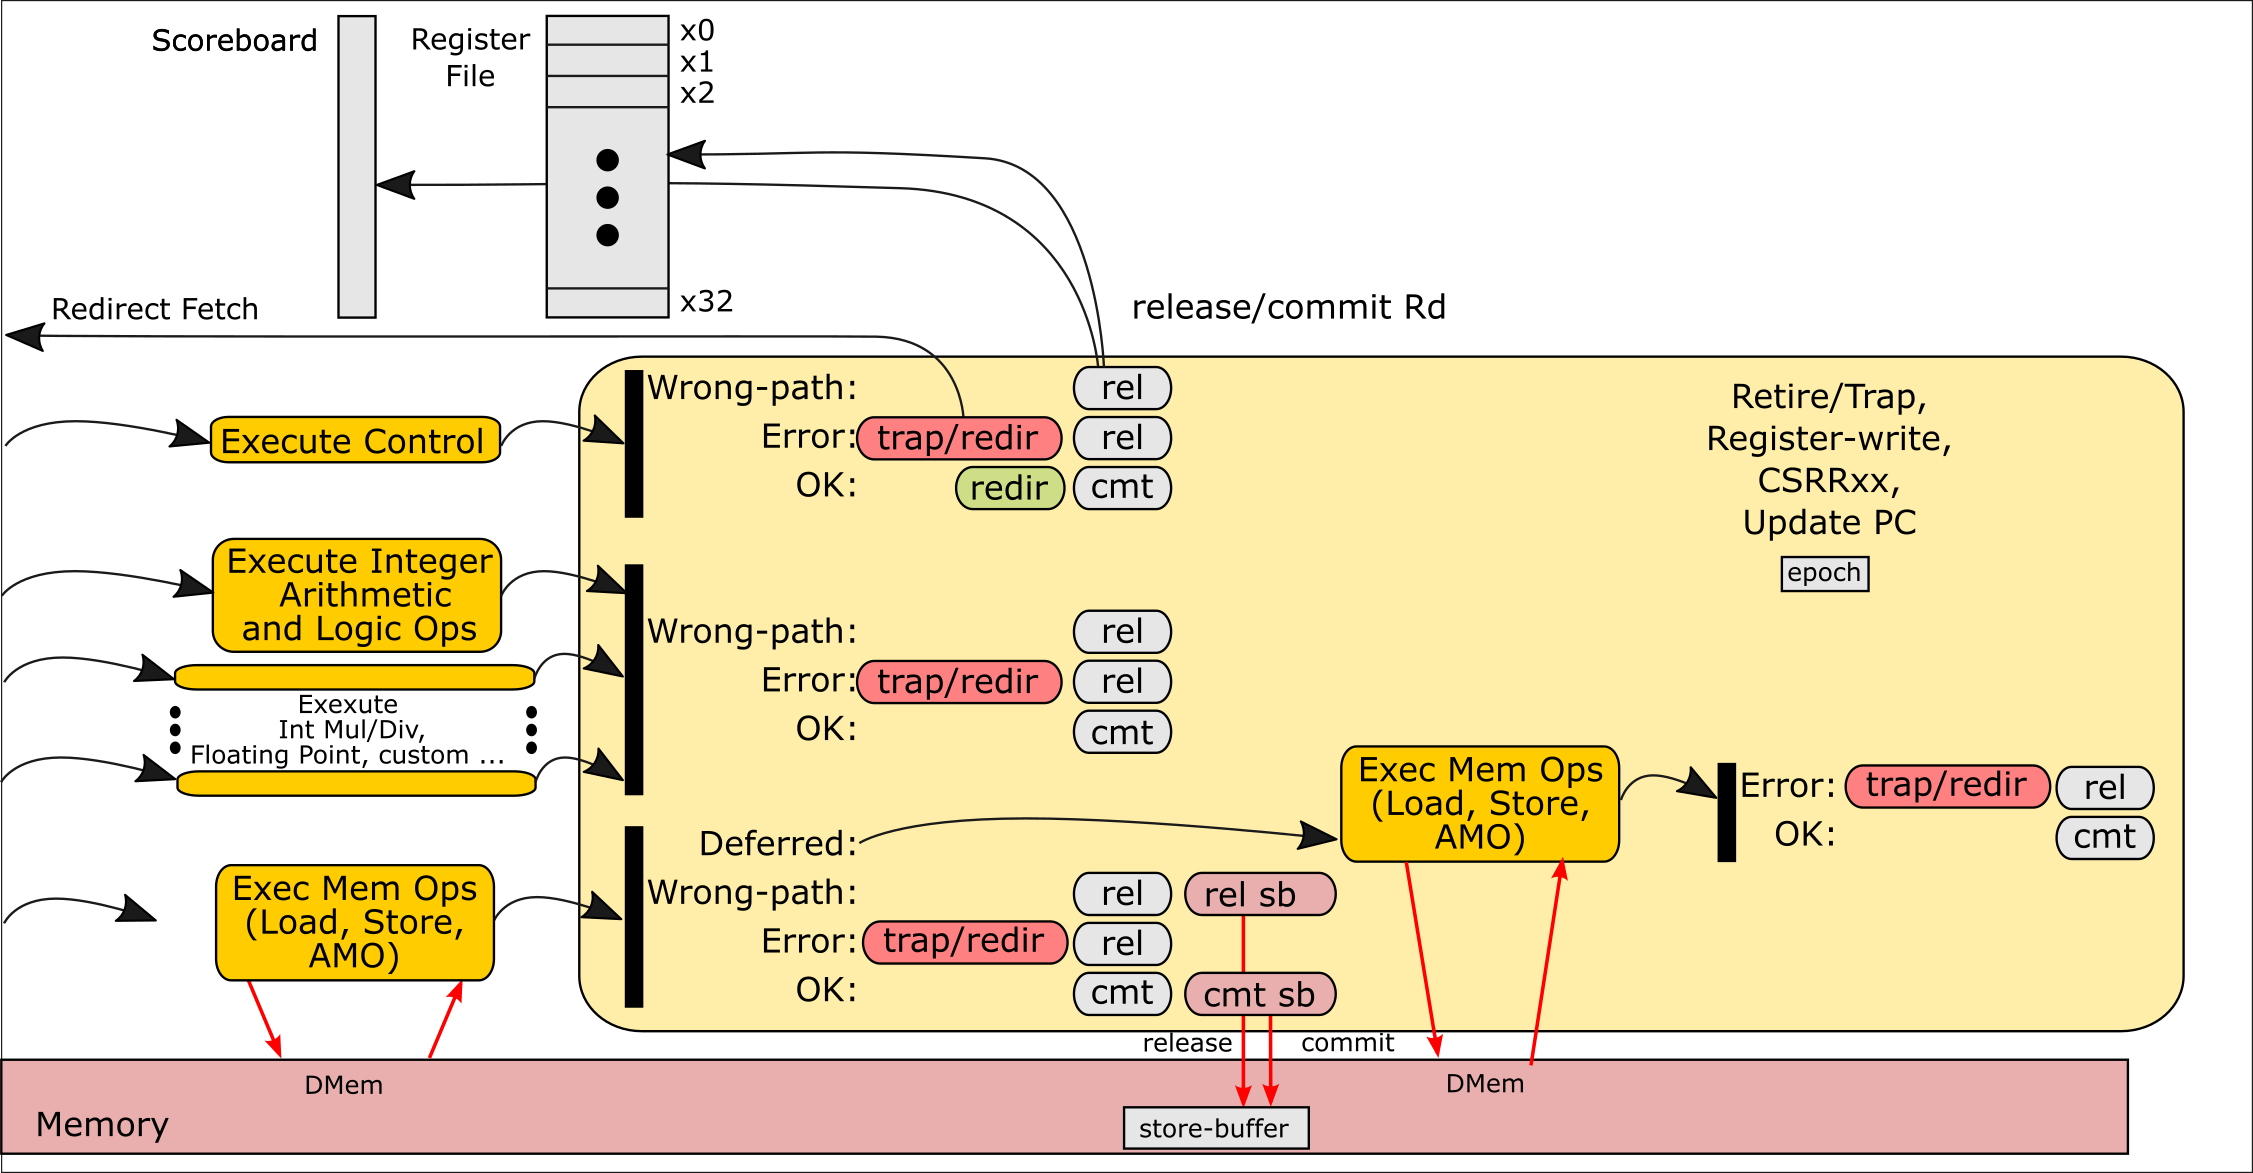
\includegraphics[width=6in,angle=0]{Figures/Fig_Fife_Retire}}
  \caption{\label{Fig_Fife_Retire}Actions in the ``Retire'' stage of Fife}
\end{figure}

% ****************************************************************

\section{Fife: CSRs}

\begin{tightlist}
\item CSRRxx are read-modify-write operations
\item CSRRxx access may not be memory-like (side-effecting reads, read
      may not return last written value,
\item ... (a bit like MMIO issues)
\end{tightlist}
Hard to pipeline, so execute in Retire stage, as FSM.

CSRRxx instructions should be rare, so FSM exec does not affect overall performance.

% ****************************************************************

\section{Fife: Interrupts}

Sample for interrupts in Retire stage, fix up CSRs and and redirect.

Retire stage already has infra for CSR update and redirection, so this
is a small incremental change.

% ****************************************************************
